\kap{Introduction}\label{chap:innledning}
%\begin{flushleft}


\section[Nucleon-Nucleon models]{Nucleon-Nucleon(NN) interactions And Nuclear Models}



Particles can be grouped into three different categories, which are leptons, baryons and mesons.
Leptons are particles like the electron and neutrino. 
Baryons are particles with half integer spin like the nucleons,
while mesons are particles with integer spin.
It is also normal to call the big group of baryons and mesons for hadrons, since they are all made from quarks.

The mesons are the carrier of the strong force. They can interact with nucleons through the strong, weak,
electromagnetic and gravitational force. Free mesons can be produced in nucleon-nucleon collisions, but they decay
rapidly into lighter mesons, leptons or photons either through strong, weak or electromagnetic interactions. 
The decay lifetimes are around $10^{-20}-10^{-23}$ for strong decays, $10^{-16}-10^{-18}$ for electromagnetic decays 
and $10^{-8}-10^{-10}$ for weak decay. In the nucleon-nucleon scattering processes we are looking at, we can
neglect all the other forces except the strong force. So the contribution to the potential created between
the nucleons are  only arising from strong interactions through virtual meson exchange.

There are many different mesons. They all have their own contribution to the strong force,
which is a superposition from all the possible ways the mesons can be exchanged. 
i.e. not only a single meson exchange, but also more complicated events where two ore more mesons are transfered.
All the mesons have their own characteristic combination of mass, spin, parity, isospin and decay rate. 
these parameters are important for the range of the force, but also for where it will be repulsive/attractive.
It is normal to divide the range of the strong force into three regions; 
The short range, the intermediate region and the long-range of the force.
For example the $\pi$-meson as the lightest particle provides the long-range force. 
While the $\omega$-meson is responsible for the short-range repulsion, which explains the observed hard core of
the nucleons when they are squeezed together. From electron scattering experiments on heavy nuclears,
one have found an average distance between the centers of the nucleons to be 1.8 fm. 
This is a too large diameter of the hard core arising from the strong force. It turns out that the Pauli 
principal is more important for nucleons hard core observed in heavy nuclears. 
A better way to determine the hard core from the strong interaction is NN data form the \state{1}{S}{0}- phase shift.
This state is chosen since it doesn't have a centrifugal barrier. i.e. the angular orbital momentum; L=0. 
From fig~\ref{fig:manypotS} we see that the phase shift turns negative/repulsive around $E_{lab}=250$ MeV.
The maximum classical orbital angular momentum $L_{max}$ is
\begin{equation}\label{eq:Lmax}
L_{max}=Rp=R\sqrt{\frac{E_{lab}M}{2}}
\end{equation}
Where R is the range/radius of the hard core and M is the mass of the nucleon.
With $L\le1$ we obtain an estimate of the radius of the hard core: 
\begin{equation}\label{eq:Lmax2}
R\le 0.6 \text{ fm}
\end{equation}
Experiments shows that the deuterium has a magnetic moment, which means that the bound nuclei is a mixture
of the S-state (L=0) and the D-state (L=2). This indicates that the strong force also contains a tensor-force
that can couple the two states with the same good quantum numbers. 
%This indicates that we need more than 
%the Klein-Gordon equation, which is the relativistic wave equation for scalar fields. 
The Klein-Gordon equation is used to calculate a potential from mesons with spin-$0$ (Yukawa potentials).
The Yukawa potential has it origin from a scalar-force.
This indicates that we need to work with more than
the Klein-Gordon equation to reproduce the tensor-force.
%, which is the relativistic wave equation for scalar fields.
The Dirac equation on the other hand will be able of handling tensor-forces, 
but is only valid for half integer spin particles like nucleons and quarks.
One must of course use field theories for spin-1, spin-2 and higher spin models.
Spin-1 theory for meson has much in common with the field theory for photons. 
Photons also have spin-1, but unlike the mesons, it has zero mass. 
It turns out that spin-1 fields can create a tensor force.
Models for the higher spin-mesons exist, but
One Boson Exchange (OBE) models, like the Bonn B potential, normally only include spin-0 and spin-1 mesons.
This approximation is good because the mesons are generally heavier as the spin increases.
The heavier mesons will only have a short range. Their contribution will be small to the strong force.
In Bonn B for example the $\sigma$-meson are supposed to be the average effect of all the heavier mesons and all the
multiple meson exchanges.
%So for the 
%Spin-1 field theories
%From definition the mesons are particles with integer spin.

%So to make a good potential of the strong interactions, one have to have in mind that mesons are made up of quarks
%with half integer spin. One also sees that the Klein Gordon equation no longer can be interpreted as a consistent
%one particle equation. 


All integer spin particles are made up of half integer spin particles. 
Handling the mesons as a particle will only give approximate theories to the real jungle.
This approximation gets worse and worse as the energy of the NN-system is increased. 
Finally the meson theory breaks down, and the system has to be dealt with as a system of quarks instead.
In OBE-models this effect is implemented as so called cutoff-parameters.

It is the strong force that holds the nucleons together in nuclears, but the Pauli principal is 
also important for the way nucleons binds and forms nuclears. 
From the decay rate we see that a meson can move a 
couple of Fermi meters before it decays through the strong force. This must off course hold for virtual mesons to. 
It is a relatively short 
range. So in a nuclear the strong force is (approximately) only active among neighboring nucleons. 
This explains why the binding energy per nucleon increases from the smallest nuclear ${}^2$H ($\sim$ 1 MeV) till 
${}^4$He ($\sim$ 7 MeV), 
and then is more stabile for larger nucleons. With a maximum at ${}^{56}$Fe ($\sim$ 8.5 MeV). 
The energy per bound is also interesting to look at.
The energy per bound is about 2 MeV for ${}^2$H, 3 MeV for the triton and 4.5 MeV for ${}^4$He. 
One can also conclude that; When nucleons are pulled closer to each other by more bonds due to more nucleons, 
but also the energy per bound increases to. This is an interesting effect created by a three body-force, which
has no classical analog.


This gives rise to different nuclear models like the liquid-drop model. 
The liquid-drop model has only the protons and the total number of nucleons as parameters.
A much better model would of course be to use the exact potential that is created through meson exchange,
and then build up the nuclears with it.
In order to do that, the first thing one needs is a model of the potential. This has led to a own branch in
nuclear physics.

Calculating the phase shifts gives an indication of the strength of the potential between the two nucleons.
If one has a good guess of how the potential must be, one can test it by running a computer program 
(like one described later) to calculate the phase shift and inelasticity. 
One can in principal check the theoretical potential with experimental values of phase shift and inelasticity,
which we now have very good experimental values for.
The One Boson Exchange (OBE)-model is such a theoretical potential.
As mentioned before, this potential contains a couple of "cutoff" parameters and a fictive $\sigma$-meson, 
which has to be adjusted to fit the experimental values as good as possible. This model gets very close to
the experimental data for low energies. But it is a little bit too steep in many cases, like it is in 
fig~\ref{fig:manypotS}. New and better models have been developed the recent years.
Charge-Dependent (CD) Bonn is one of them ~\cite{cd-bonn}. 
This model is building on the OBE model but is using charge dependents, i.e. u and d quarks has different masses.
This model can reproduce almost exact results for lab energies below 300 MeV, 
when it is fitted with experimental data. This is a good indication of the isospin dependence of the strong force,
and indicates that the meson-theory is good. It is actually so good that Machleidt, my supervisor here in USA 
who worked on the CD-Bonn potential, has focused his interest in solving the higher energy models instead. 
These models has to account on more complex meson exchanges, excitations of the nucleons, 
and even production of other particles.
The new high energy models also include properties taken from quantum chromodynamics (QCD).
%The next step for these models seems to be
Like confinement and chiral perturbation, which seems to be the next step in modeling the strong force.

The meson theory has been developed from a wish to understand the basic force holding the nucleons together. 
When the meson-model work well compared with it's limited accuracy, one will have to try to solve the "real" problem. 
i.e. leaving the mesons and nucleon, which is a sort of an approximation of how the quarks behavior.
Such quark models are still far from being good, but hopefully it will be worked out one day. 

%The next step now seems to be confinement and chiral
%perturbation models, which is mostly  the old meson theory, but includes properties of quantum chromodynamics (QCD). 

The meson model has been polished for quite a time now, and is the best model we have of
the strong interaction.
But even with a good potential model of the strong force, it is difficult to apply it to nuclears. 
The strong force is a three body force. That is, the force on nucleon 1 not only depends on the individual
position of nucleon 2 and 3, it contains an additional contribution that arises from the correlation 
of the positions of nucleon 2 and 3. 
Solving this problem exact is difficult for heavy nuclears since it is dependent on all the nucleons position in the nuclear.
The mathematic is complicated and one loose physical insight.

People have compared this model with describing a gas by how all the molecule move, rather than using a few parameters such as 
pressure and temperature. They want to use oversimplified theories like  "shell models" to describe nuclears. 
This theory is mathematically easy to work with and gives a good physical insight. 
One can for example see from this theory that the strong interaction must include a spin-orbit force and a
spin-spin ($\sigma\cdot\sigma$) force. But these forces can also be studied in 
NN-scattering. For example can the spin-orbit
force be observed in pp-scattering experiments with the triplet P waves. 

The nuclear science has been divided by different models.
This way the theoretical nuclear group in Oslo and Bergen have ended up working with two different theories even though 
they work with the exact same problem.  

\section{Phase Shift For Partial Waves} 

As mentioned already, phase shifts are very important for the understanding of the strong force.
Phase shift $\delta_l$ is a result from the de Broglies postulate, which states that particles also behaves as waves.
Particles have  a wave length $\lambda$, called de Broglie wavelength related to the particle's momentum p as
\begin{equation}\label{eq:Broglie}
\lambda=\frac{2\pi\hbar}{p}
\end{equation}
$\lambda$ will therefor be dependent on the energy of the particle/(wave packet). This is illustrated
in fig~\ref{fig:ilusterendeFaseskift}. Note that $\lambda$=$\pi\delta$, where $\delta$ is the phase shift.
\begin{flushleft}   
\begin{figure}\label{fig:ilusterendeFaseskift}
\centering
\includegraphics[height=15cm,angle=-90]{detteerfaseskift.eps}
\caption{Shows how a wave function will behave for a attractive box potential. The dashed line
illustrates the wave function behavior with out the potential.}
\end{figure}
\end{flushleft} 
However the phase shift can not be found directly. Experimentalist have to study the observable, 
which can be for example differential cross section and polarization. With these data, theorists are
able to calculate an NN-amplitude (A) for the process. This amplitude has many of the same properties as the S-matrix,
like the unitarian. In partial wave decomposition, it is related to the phase shift $\delta_l$ as
\begin{equation}
A_l=\eta_l e^{i2\delta_l}
\end{equation}

Inelasticity ($\eta_l$) is the probability amplitude for the scattering amplitude to be elastic. 
The inelasticity and phase shift are the necessary parameters to describe a partial wave. The inelasticity
becomes important for NN-scattering when the kinetic energy in the lab-system are above 350 MeV.
The inelasticity are due to energy released from the NN-system. This can be done by photon emission and/or particle
creations in the scattering.

  
%fig~\ref{fig:manypotS} shows the phase shift for different potentials and experimental phase shift.
%How the potentials are build up will be explained later.



\begin{flushleft} 

\begin{figure}\label{fig:manypotS}
\centering
\includegraphics[height=17cm]{manypotS.eps} 
\caption{\state{1}{S}{0} phase shifts for a box Potential, a parameterized potential, the Bonn B potential and
experimental data ~\cite{PRC48faseskift350MeV}. How the potentials are build up will be explained later.}
\end{figure}


\end{flushleft}


